\section{Simulation Results and Analysis} \label{sec:SimulationResultsAnalysis}

This section presents the analysis of the simulation results. A simulated scenario is considered successful if the resulting implied volatility surface satisfies all five quality criteria introduced in Section~\ref{subsec:SimulationQualityCriteria}. These criteria are motivated by empirical stylized facts observed in financial markets and are designed to assess whether a simulated surface can be regarded as realistic.

First, the quality criteria are formally defined. Next, a ceteris paribus analysis is conducted to isolate the effect of individual model parameters. Finally, the simulation output is evaluated across a broad set of parameter constellations, and parameter ranges with high success rates are identified.


\subsection{Simulation Quality Criteria} \label{subsec:SimulationQualityCriteria}

Based on empirical observations in financial markets, five quality criteria are defined to assess the plausibility of simulated implied volatility surfaces:
\begin{itemize}
    \item Put-call parity must hold.
    \item The implied volatility smile must exhibit convexity.
    \item The at-the-money (ATM) volatility skew should be negative.
    \item The ATM skew should increase with time to maturity.
    \item The ATM skew term structure should decay approximately according to a power law.
\end{itemize}
A simulation scenario is considered successful if the resulting implied volatility surface satisfies all five quality criteria.

\subsubsection*{Put-Call Parity Criterion}
The put-call parity (see \citealp{Björk2009}) establishes a fundamental no-arbitrage relationship between the prices of European call and put options. At time $t$, it states:
\begin{equation} \label{eq:PutCallParity}
    C_t - P_t = S_t - K \cdot B(t,T),
\end{equation}
where $C_t$ and $P_t$ denote the prices of a European call and put option with strike $K$ and maturity $T \geq t$, $S_t$ is the spot price of the underlying asset, and $B(t,T) = e^{-r(T - t)}$ is the discount factor under a constant risk-free rate $r$.

In the simulation, this relation is evaluated at $t = 0$. The element-wise relative deviation from parity is computed as:
\begin{equation} \label{eq:PutCallViolation}
    \text{Relative Error}_{l,q} = \left| \frac{C_0^{(l,q)} - P_0^{(l,q)} - \left( S_0 - K_l e^{-r T_q} \right)}{S_0} \right|,
\end{equation}
where the indices $(l, q)$ refer to strike $K_l$ and maturity $T_q$.

The criterion is satisfied if the mean relative deviation across all $(l, q)$ does not exceed 0.1\% and the maximum deviation does not exceed 0.5\%. Meeting this condition ensures internal consistency between simulated call and put prices, allowing them to be aggregated into a single implied volatility surface.

\subsubsection*{Smile Convexity Criterion}
In financial markets, implied volatility typically exhibits a smile-shaped pattern across strikes for a fixed maturity: it tends to be lowest at-the-money and higher for deep in- or out-of-the-money options. To assess convexity, a quadratic polynomial is fitted to the implied volatilities for each maturity.

The criterion is satisfied if the fitted parabola has a positive leading coefficient and an $R^2$ value above 90\%. This convex smile pattern must be observed for the shortest maturity and for at least 90\% of all maturities overall.

\subsubsection*{ATM Skew Negativity Criterion}
Empirically, the ATM volatility skew tends to be negative, meaning that implied volatility decreases with increasing moneyness around the at-the-money level. The ATM skew is defined as in \citet{BayerFrizGatheral2016} by
\begin{equation} \label{eq:ATMSkew}
    \psi(\tau) := \left. \frac{\partial}{\partial k} \sigma_{\text{BS}}(k, \tau) \right|_{k = 0},
\end{equation}
where $\sigma_{\text{BS}}(k, \tau)$ is the implied Black-Scholes volatility for log-moneyness $k$ and maturity $\tau$.

The criterion is satisfied if $\psi(\tau) < 0$ for at least 90\% of the maturities.

\subsubsection*{ATM Skew Increase Criterion}
It is commonly observed that the magnitude of the ATM skew diminishes with increasing maturity, resulting in a flatter term structure. Hence, the ATM skew function $\psi(\tau)$ is expected to increase with maturity, i.e., become less steep for longer maturities.

The criterion is satisfied if a linear regression of $\psi(\tau)$ against maturity yields a positive slope.

\subsubsection*{ATM Skew Power Law Criterion}
Empirical studies suggest that the ATM skew decays approximately as a power law (see \citealp{Fukasawa2011} and \citealp{GatheralJaissonRosenbaum2018}) of the form:
\begin{equation} \label{eq:PowerLaw}
    \psi(\tau) \sim \tau^{-\gamma},
\end{equation}
with $\gamma = \tfrac{1}{2} - H$. The criterion is satisfied if a linear regression on the log-log plot of $\psi(\tau)$ versus $\tau$ achieves an $R^2$ value greater than 90\%.


\subsection{Effects of Individual Parameters} \label{subsec:IndividualParameterEffects}

This section analyzes how varying one model parameter, while keeping all others fixed, affects the shape of the implied volatility surface and the performance with respect to the simulation quality criteria. The analysis is conducted in a ceteris paribus fashion and provides intuition for the results of the full parameter sweep presented in later sections.

\subsubsection*{Effect of the Roughness Parameter $H$}
For lower values of $H$ (i.e., rougher sample paths), the short-term ATM skew decreases in magnitude. Additionally, the slope of the log-log regression fitted to the ATM skew term structure flattens, indicating that the power-law exponent decreases in absolute value as $H$ decreases.
\begin{figure}[H]
    \centering
    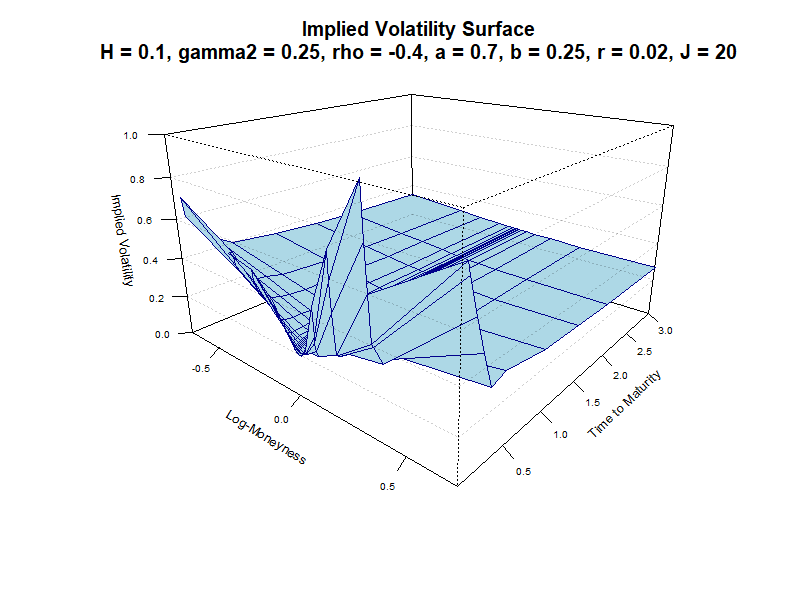
\includegraphics[width=0.45\textwidth]{figures/5.2 Individual Parameter Effects/H=0.10_iv_surface.png}
	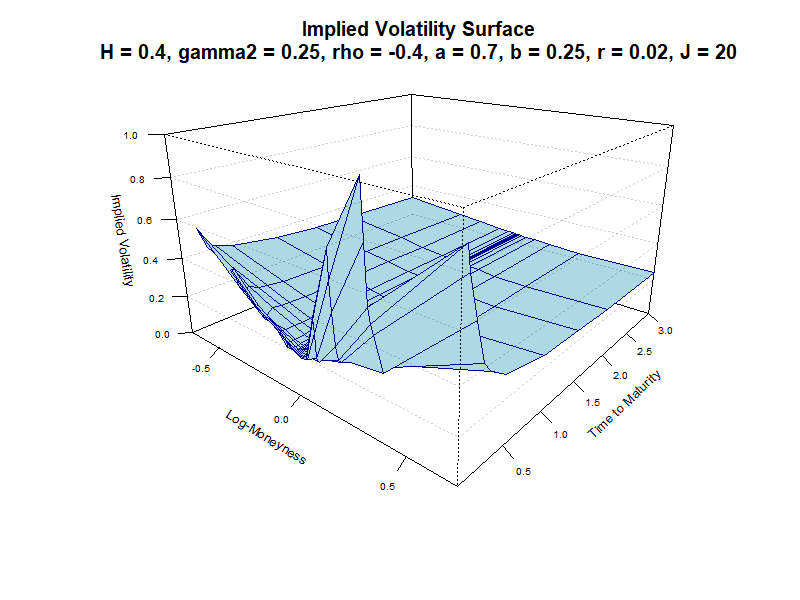
\includegraphics[width=0.45\textwidth]{figures/5.2 Individual Parameter Effects/H=0.40_iv_surface.png}
	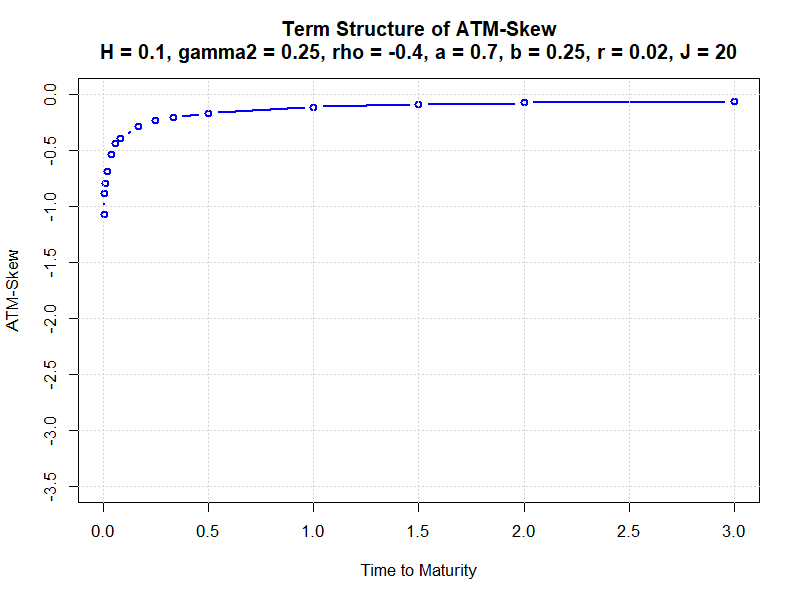
\includegraphics[width=0.45\textwidth]{figures/5.2 Individual Parameter Effects/H=0.10_atm_skew.png}
	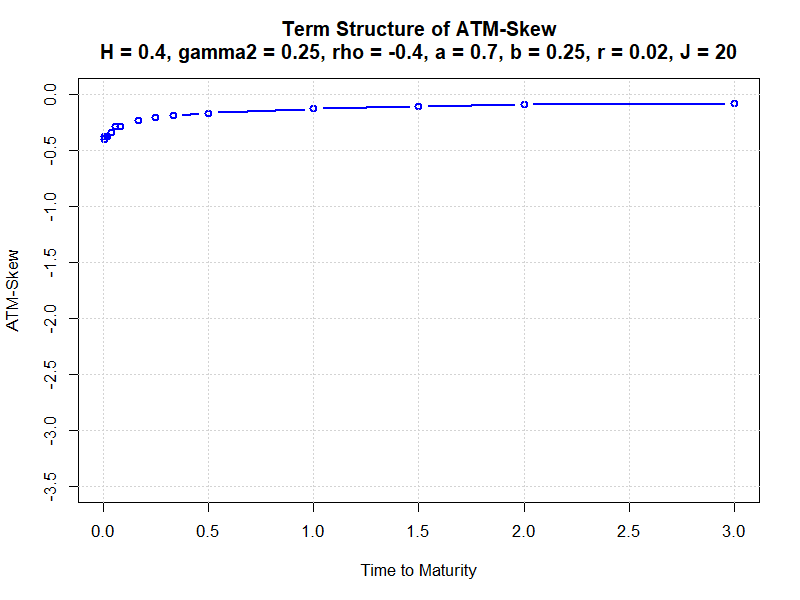
\includegraphics[width=0.45\textwidth]{figures/5.2 Individual Parameter Effects/H=0.40_atm_skew.png}
    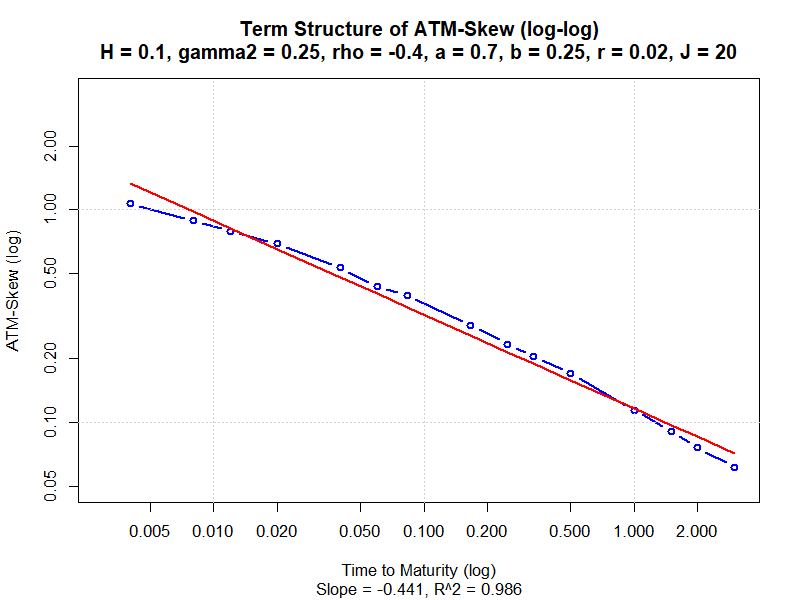
\includegraphics[width=0.45\textwidth]{figures/5.2 Individual Parameter Effects/H=0.10_atm_skew_log.png}
	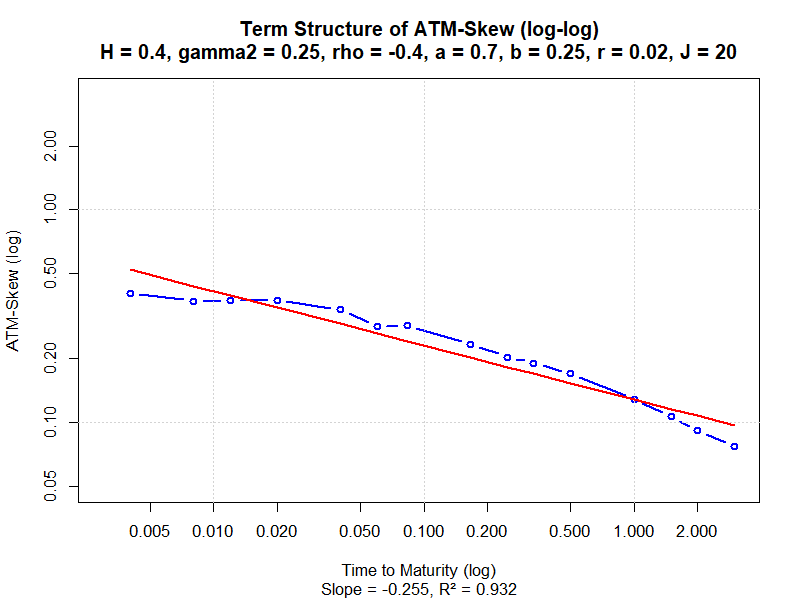
\includegraphics[width=0.45\textwidth]{figures/5.2 Individual Parameter Effects/H=0.40_atm_skew_log.png}
    \caption{Effect of roughness index $H$ on the implied volatility surface. Left: $H=0.10$. Right: $H=0.40$.}
    \label{fig:H_effect}
\end{figure}

\subsubsection*{Effect of Persistence Parameter $\gamma_2$}
\begin{minipage}{\textwidth}
Higher values of $\gamma_2$ increase the persistence in the signal process. This reduces the short-term ATM skew and flattens the power-law slope in the log-log skew regression. Overall, increased persistence slightly lowers the implied volatility surface, especially at short maturities.
\begin{figure}[H]
    \centering
    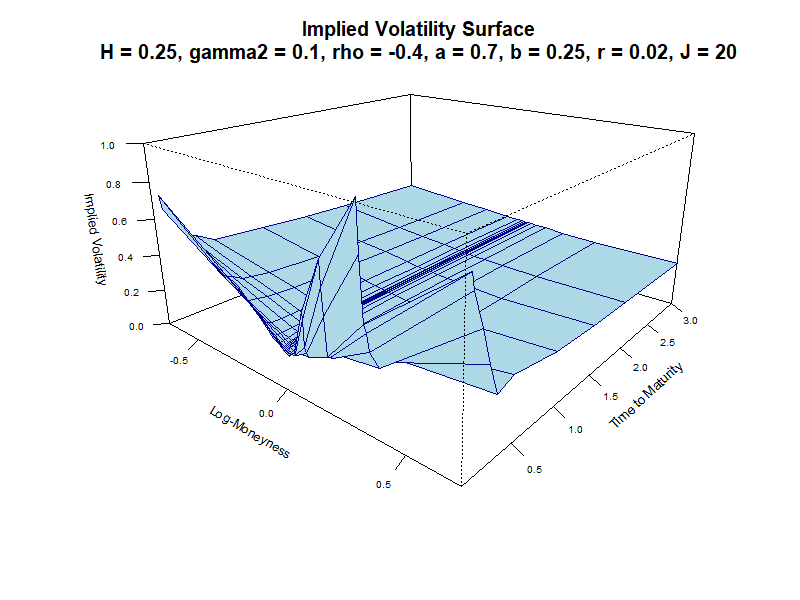
\includegraphics[width=0.45\textwidth]{figures/5.2 Individual Parameter Effects/gamma2=0.10_iv_surface.png}
	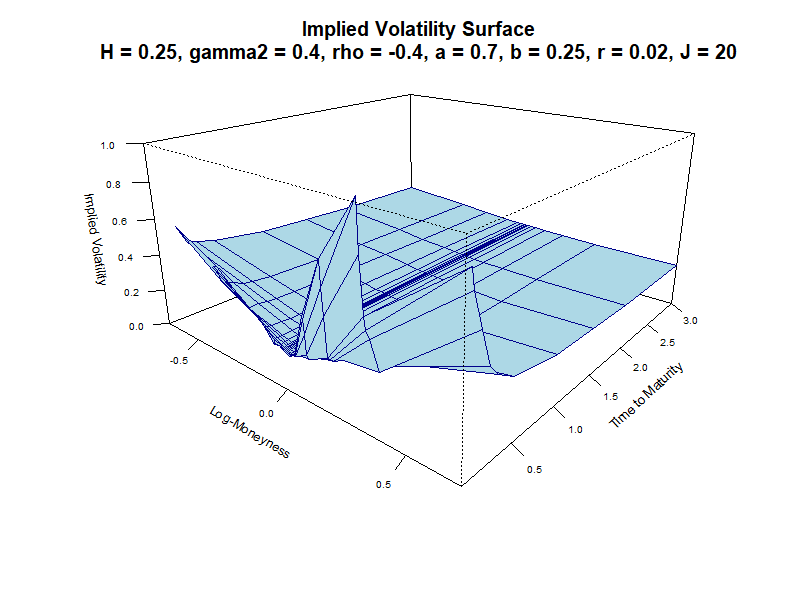
\includegraphics[width=0.45\textwidth]{figures/5.2 Individual Parameter Effects/gamma2=0.40_iv_surface.png}
	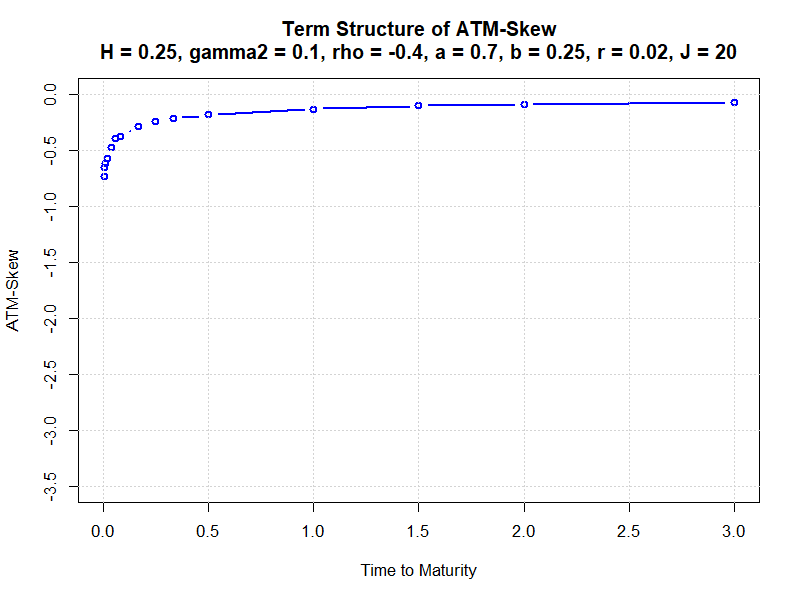
\includegraphics[width=0.45\textwidth]{figures/5.2 Individual Parameter Effects/gamma2=0.10_atm_skew.png}
	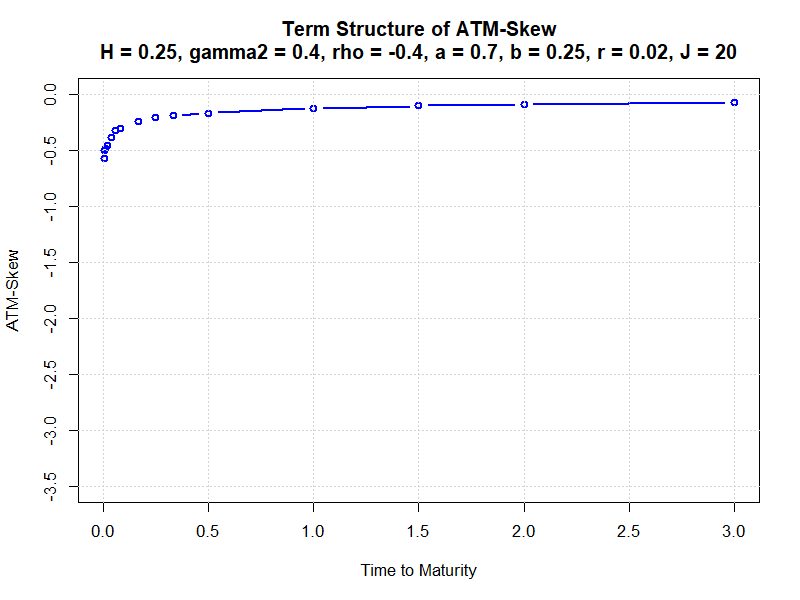
\includegraphics[width=0.45\textwidth]{figures/5.2 Individual Parameter Effects/gamma2=0.40_atm_skew.png}
    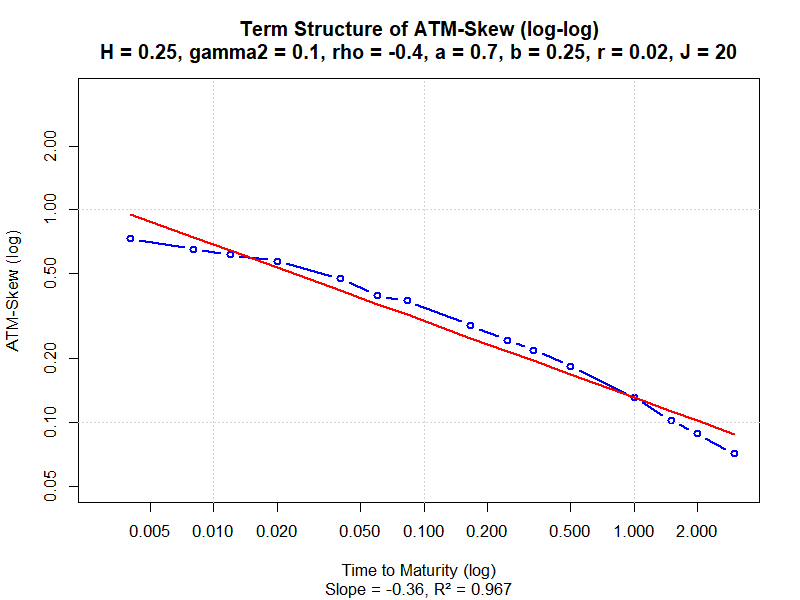
\includegraphics[width=0.45\textwidth]{figures/5.2 Individual Parameter Effects/gamma2=0.10_atm_skew_log.png}
	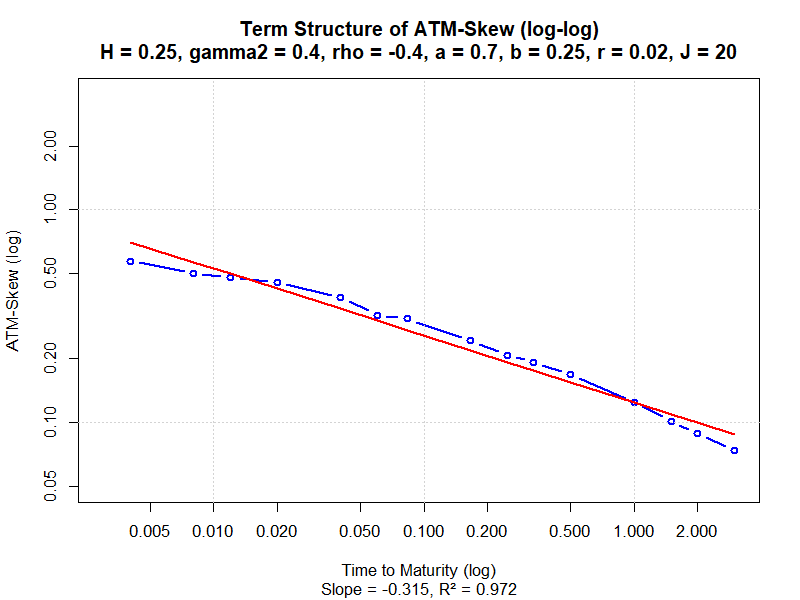
\includegraphics[width=0.45\textwidth]{figures/5.2 Individual Parameter Effects/gamma2=0.40_atm_skew_log.png}
    \caption{Effect of persistence parameter $\gamma_2$ on the implied volatility surface. Left: $\gamma_2=0.10$. Right: $\gamma_2=0.40$.}
    \label{fig:gamma2_effect}
\end{figure}
\end{minipage}

\subsubsection*{Effect of Correlation Parameter $\rho$}
\begin{minipage}{\textwidth}
Increasing the correlation $\rho$ between the Brownian motions driving the asset price and the volatility process (i.e., reducing the leverage effect) tilts the implied volatility surface to the left. This results in lower implied volatilities for positive log-moneyness and higher volatilities for negative log-moneyness. As a consequence, the magnitude of the ATM skew increases.
\begin{figure}[H]
    \centering
    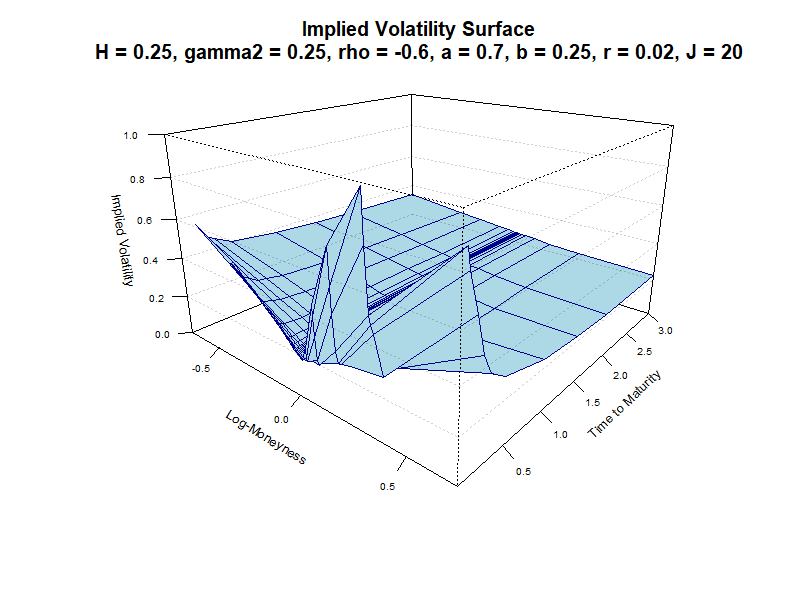
\includegraphics[width=0.45\textwidth]{figures/5.2 Individual Parameter Effects/rho=-0.6_iv_surface.png}
	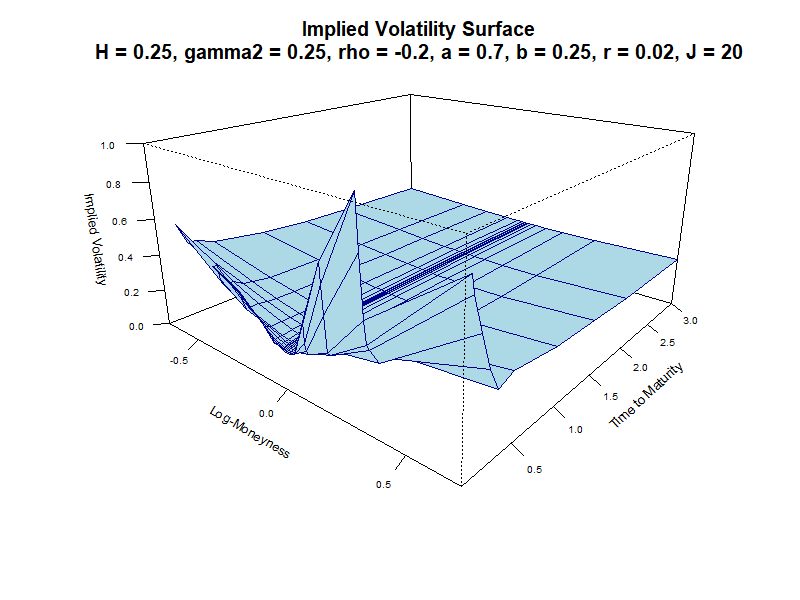
\includegraphics[width=0.45\textwidth]{figures/5.2 Individual Parameter Effects/rho=-0.2_iv_surface.png}
	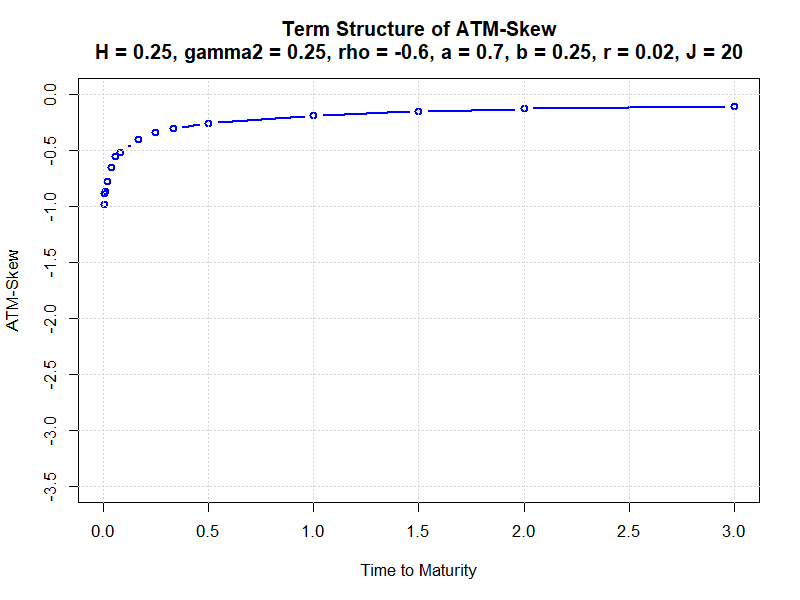
\includegraphics[width=0.45\textwidth]{figures/5.2 Individual Parameter Effects/rho=-0.6_atm_skew.png}
	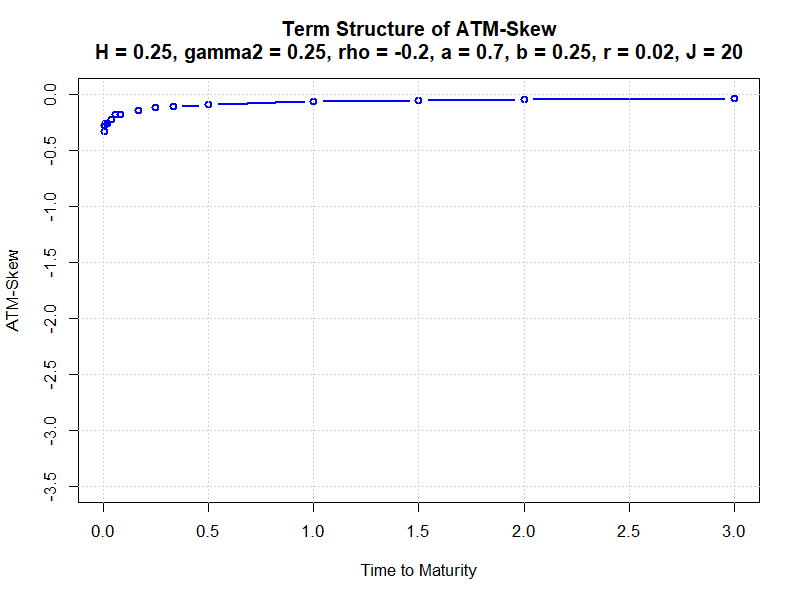
\includegraphics[width=0.45\textwidth]{figures/5.2 Individual Parameter Effects/rho=-0.2_atm_skew.png}
    \caption{Effect of correlation $\rho$ on the implied volatility surface. Left: $\rho=-0.6$. Right: $\rho=-0.2$.}
    \label{fig:rho_effect}
\end{figure}
\end{minipage}

\subsubsection*{Effect of Volatility Scale Parameter $a$}
\begin{minipage}{\textwidth}
Increasing the volatility scale parameter $a$ amplifies the influence of the latent signal process on the volatility level. This leads to higher implied volatilities in the wings, i.e., for deep in- or out-of-the-money options. The ATM skew magnitude also increases, particularly for short maturities.
\begin{figure}[H]
    \centering
    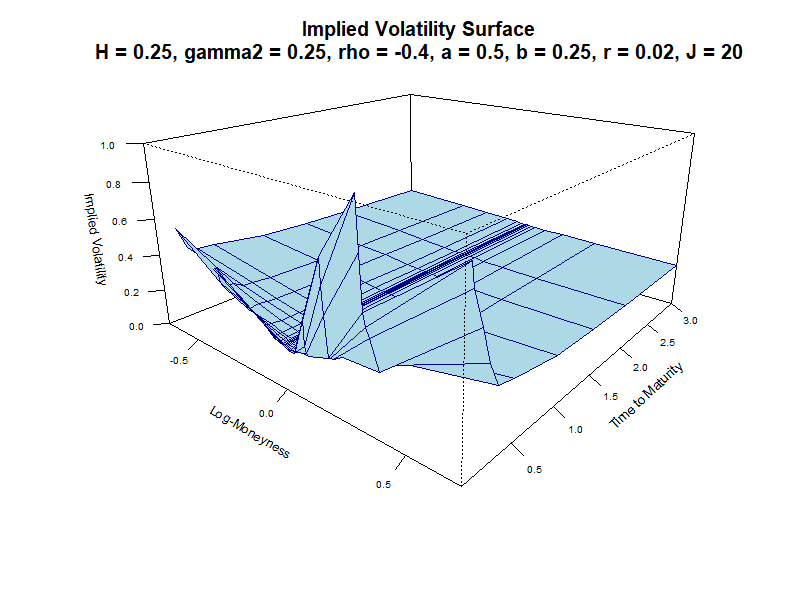
\includegraphics[width=0.45\textwidth]{figures/5.2 Individual Parameter Effects/a=0.5_iv_surface.png}
	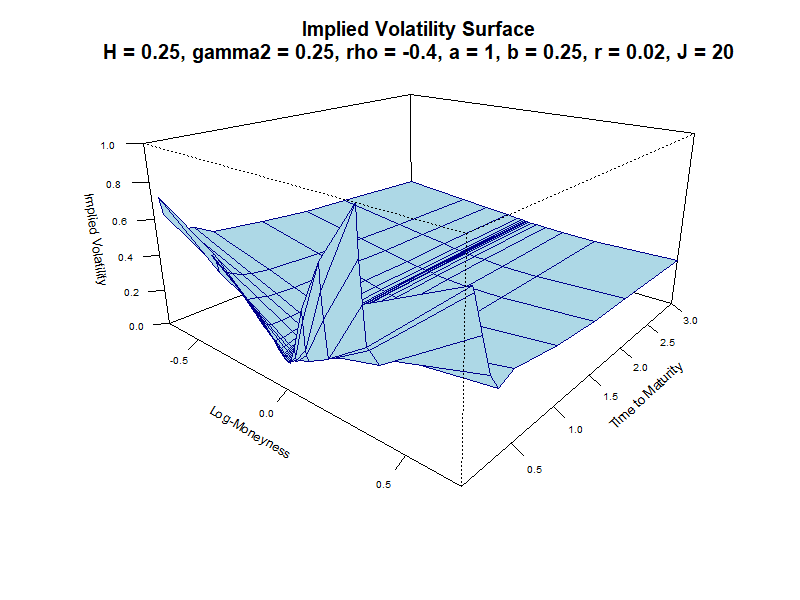
\includegraphics[width=0.45\textwidth]{figures/5.2 Individual Parameter Effects/a=1.0_iv_surface.png}
	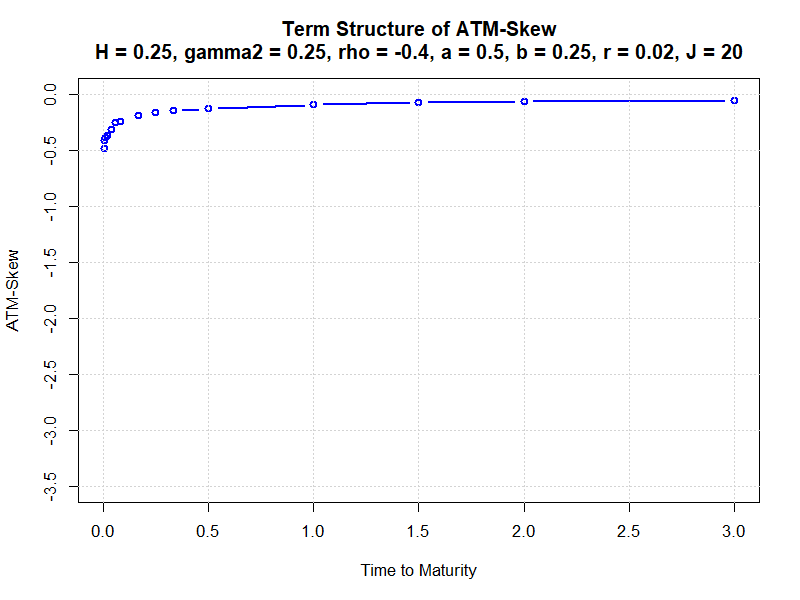
\includegraphics[width=0.45\textwidth]{figures/5.2 Individual Parameter Effects/a=0.5_atm_skew.png}
	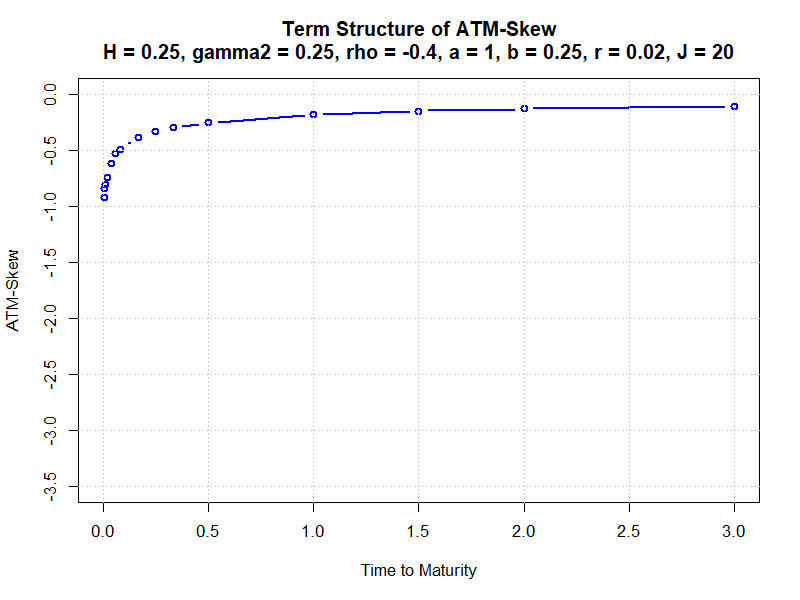
\includegraphics[width=0.45\textwidth]{figures/5.2 Individual Parameter Effects/a=1.0_atm_skew.png}
    \caption{Effect of volatility scale parameter $a$ on the implied volatility surface. Left: $a=0.5$. Right: $a=1.0$.}
    \label{fig:a_effect}
\end{figure}
\end{minipage}

\subsubsection*{Effect of Base Volatility Level $b$}
\begin{minipage}{\textwidth}
Raising the base volatility level $b$ shifts the entire implied volatility surface upward. Additionally, it increases the magnitude of the slope in the log-log regression of the ATM skew, suggesting a steeper power-law decay and hence a stronger term-structure effect in the skew.
\begin{figure}[H]
    \centering
    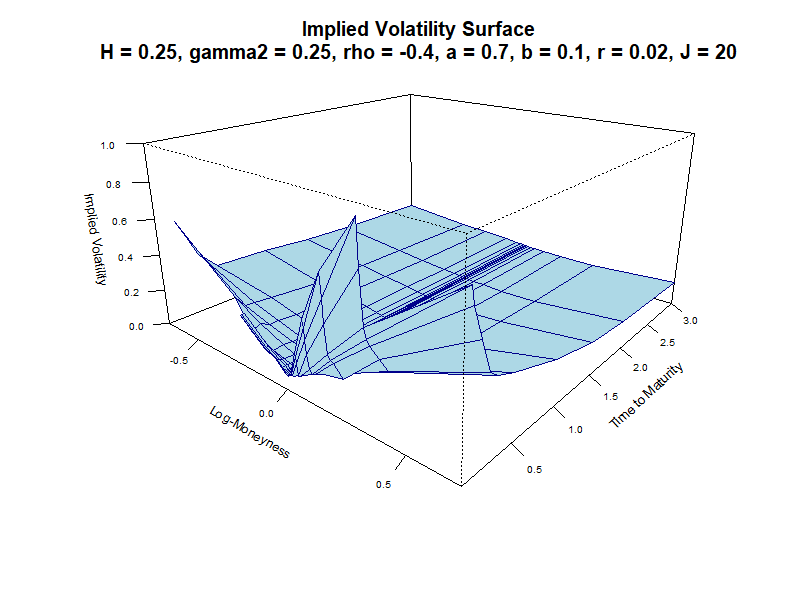
\includegraphics[width=0.45\textwidth]{figures/5.2 Individual Parameter Effects/b=0.1_iv_surface.png}
	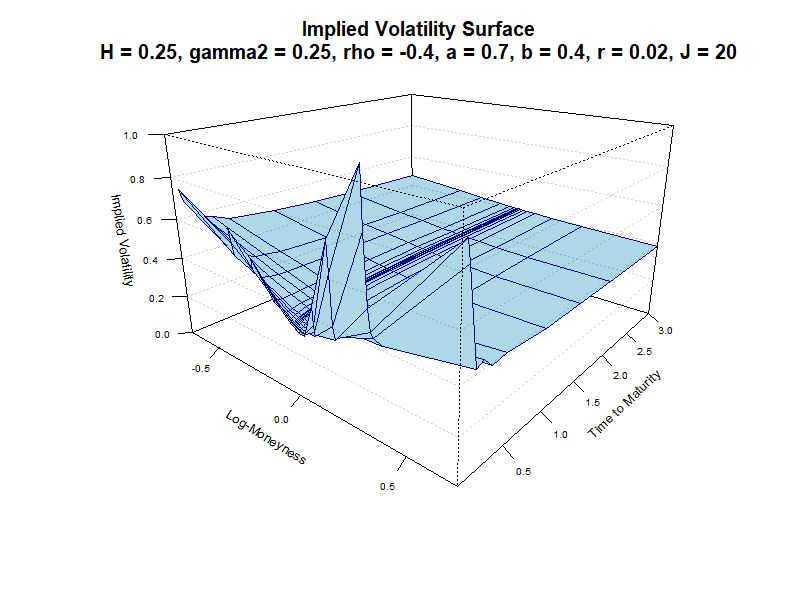
\includegraphics[width=0.45\textwidth]{figures/5.2 Individual Parameter Effects/b=0.4_iv_surface.png}
	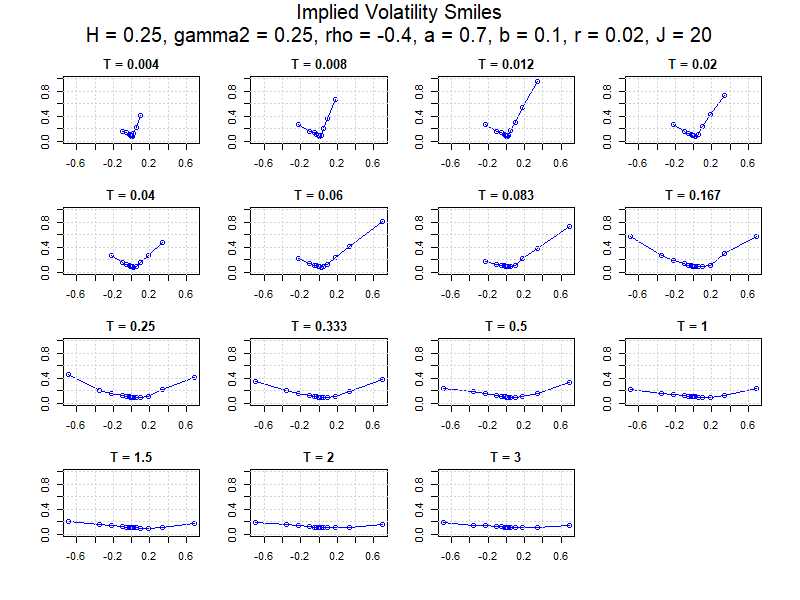
\includegraphics[width=0.45\textwidth]{figures/5.2 Individual Parameter Effects/b=0.1_iv_smiles.png}
	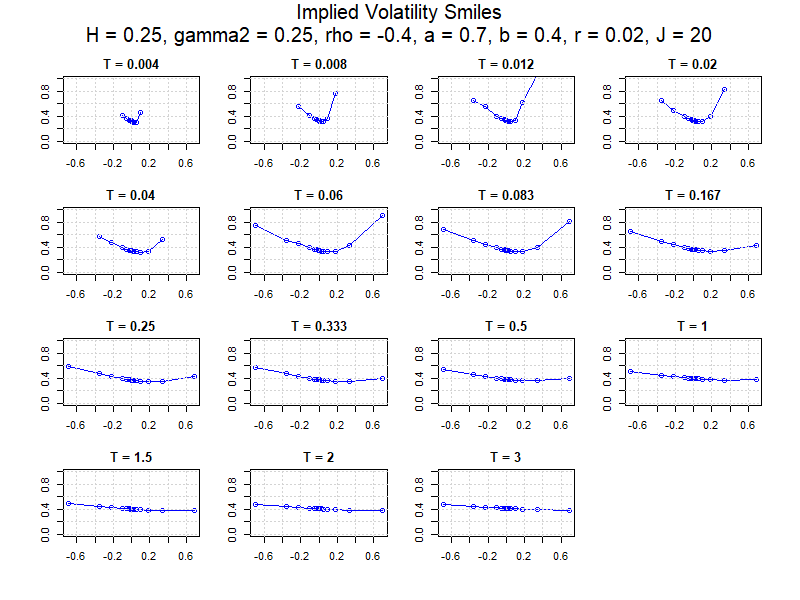
\includegraphics[width=0.45\textwidth]{figures/5.2 Individual Parameter Effects/b=0.4_iv_smiles.png}
    \caption{Effect of base volatility level $b$ on the implied volatility surface. Left: $b=0.1$. Right: $b=0.4$.}
    \label{fig:b_effect}
\end{figure}
\end{minipage}

\subsubsection*{Effect of Risk-Free Interest Rate $r$}
\begin{minipage}{\textwidth}
Changes in the risk-free interest rate $r$ have no effect on the implied volatility surface, as expected under risk-neutral pricing. This serves as a consistency check for the numerical implementation.
\begin{figure}[H]
    \centering
    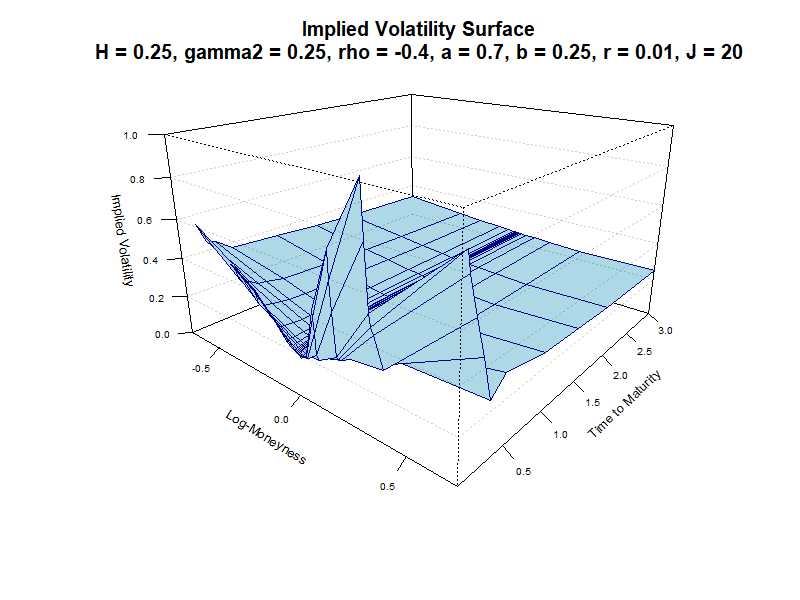
\includegraphics[width=0.45\textwidth]{figures/5.2 Individual Parameter Effects/r=0.01_iv_surface.png}
	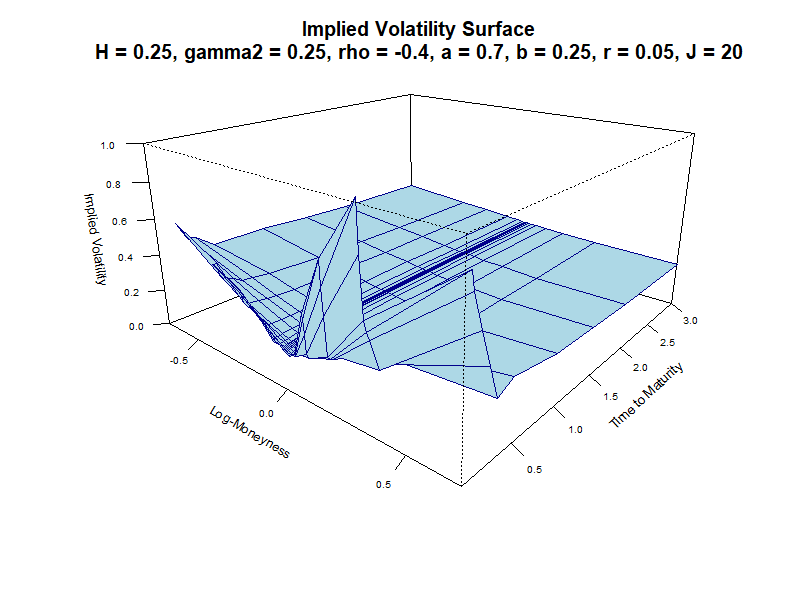
\includegraphics[width=0.45\textwidth]{figures/5.2 Individual Parameter Effects/r=0.05_iv_surface.png}
	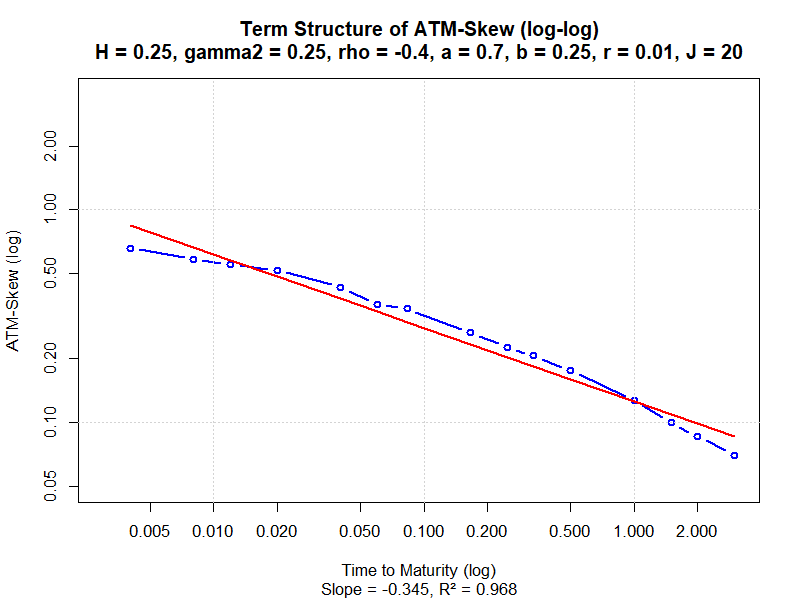
\includegraphics[width=0.45\textwidth]{figures/5.2 Individual Parameter Effects/r=0.01_atm_skew_log.png}
	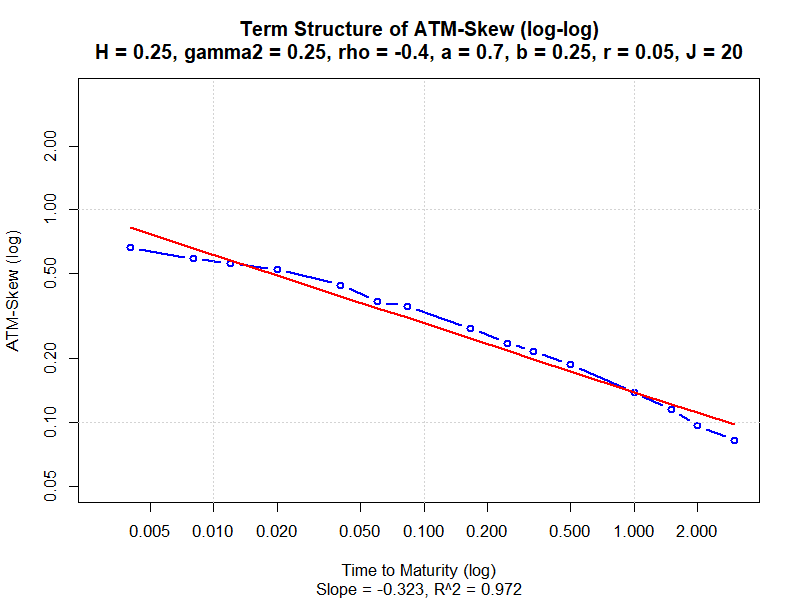
\includegraphics[width=0.45\textwidth]{figures/5.2 Individual Parameter Effects/r=0.05_atm_skew_log.png}
    \caption{Effect of risk-free interest rate $r$ on the implied volatility surface. Left: $r=0.01$. Right: $r=0.05$.}
    \label{fig:r_effect}
\end{figure}
\end{minipage}

\subsubsection*{Effect of Approximation Parameter $J$}
\begin{minipage}{\textwidth}
The stability of the simulation depends on the level of approximation of the signal process. As $J$ increases, the at-the-money (ATM) skew becomes more pronounced, indicating that a finer approximation of the rough volatility process allows the power-law behavior of the ATM skew term structure to emerge more clearly, particularly for very short maturities.
\begin{figure}[H]
    \centering
    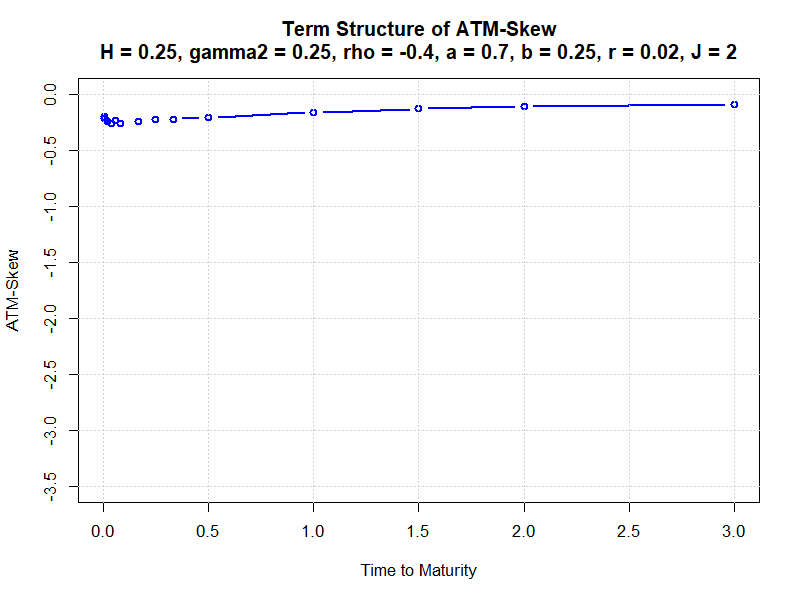
\includegraphics[width=0.45\textwidth]{figures/5.2 Individual Parameter Effects/J=2_atm_skew.png}
    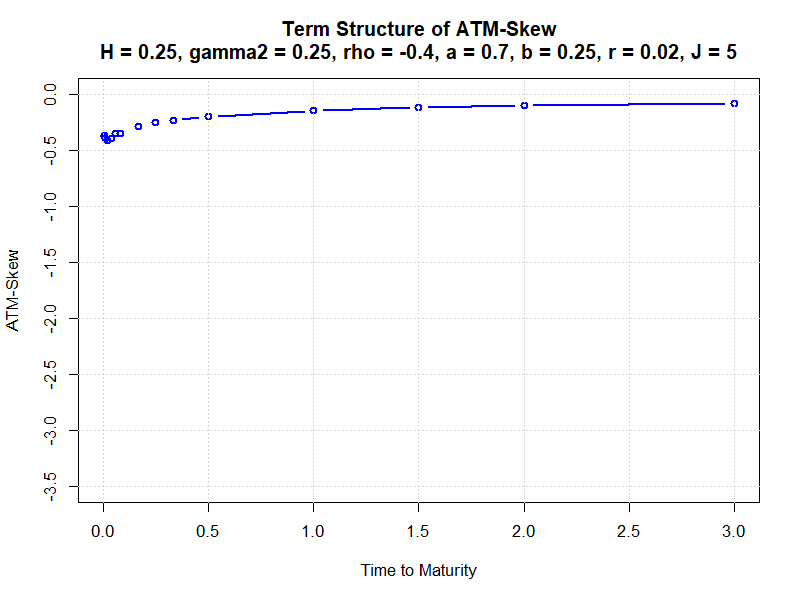
\includegraphics[width=0.45\textwidth]{figures/5.2 Individual Parameter Effects/J=5_atm_skew.png}
    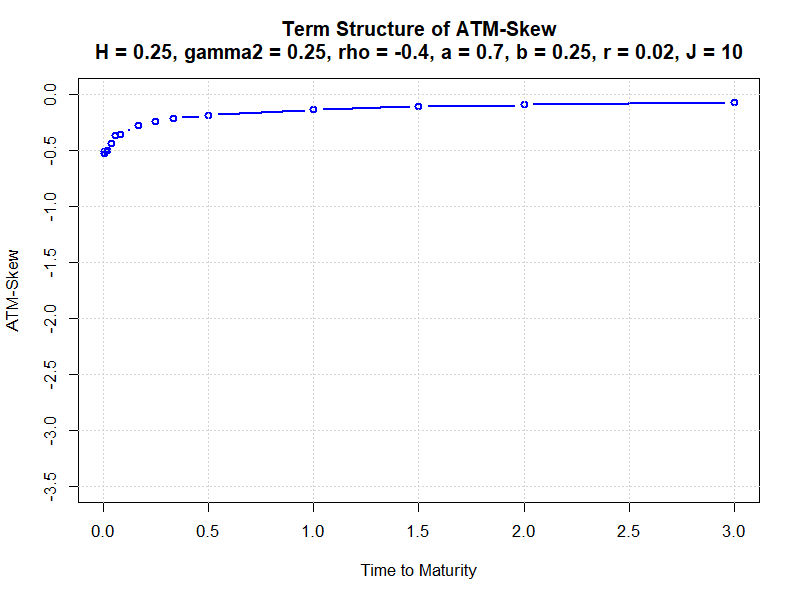
\includegraphics[width=0.45\textwidth]{figures/5.2 Individual Parameter Effects/J=10_atm_skew.png}
    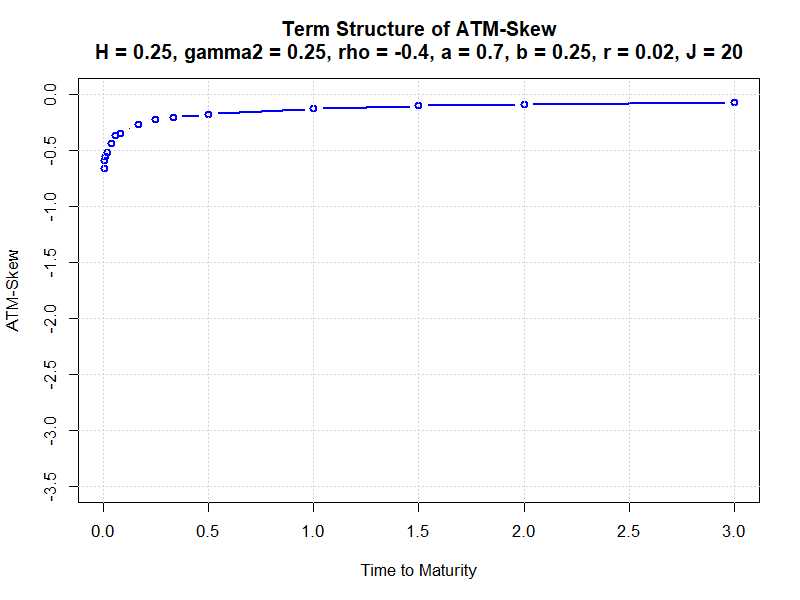
\includegraphics[width=0.45\textwidth]{figures/5.2 Individual Parameter Effects/J=20_atm_skew.png}
    \caption{Effect of approximation parameter $J$ on the ATM implied volatility skew. Top-left to bottom-right: $J=2,5,10,20$.}
    \label{fig:J_effect}
\end{figure}
\end{minipage}


\newpage
\subsection{Success Rate Analysis} \label{subsec:SuccessRateAnalysis}

To evaluate model performance, this section analyzes the proportion of simulation scenarios that satisfy the five quality criteria defined in Section~\ref{subsec:SimulationQualityCriteria}. Each scenario corresponds to a unique configuration of model parameters, and is simulated using 100{,}000 Monte Carlo paths to generate the asset price dynamics required for option pricing. A scenario is considered successful if all five criteria are met.

\subsubsection*{Parameter Grid Used in the Simulation Study}
The simulation study was based on a broad parameter grid chosen to reflect realistic variation in volatility dynamics. In total, 18{,}225 scenarios were evaluated with the following parameter values:
\begin{itemize}
    \item Roughness index $H \in \{0.05, 0.10, 0.15, 0.20, 0.25, 0.30, 0.35, 0.40, 0.45\}$
    \item Persistence parameter $\gamma_2 \in \{0.05, 0.10, 0.15, 0.20, 0.25, 0.30, 0.35, 0.40, 0.45\}$
    \item Correlation $\rho \in \{-0.8, -0.7, -0.6, -0.5, -0.4, -0.3, -0.2, -0.1, 0\}$
    \item Volatility scale parameter $a \in \{0.5, 0.7, 1.0, 1.4, 2.0\}$
    \item Base volatility level $b \in \{0.10, 0.15, 0.20, 0.25, 0.30\}$
\end{itemize}
The risk-free rate $r$ and the approximation parameter $J$ are kept constant at $r = 0.02$ and $J = 20$. The short-term parameter $\gamma_1$ was computed as $\gamma_1 = H + \tfrac{1}{2} - \gamma_2$ according to Equation~\eqref{eq:HurstIndex}, ensuring the correct asymptotic behavior of the hypergeometric kernel.

\subsubsection*{Overall Success Rates}
Put-call parity is satisfied in 93\% of simulations, smile convexity in 66\%, skew negativity in 99\%, skew increase in 96\%, and the power-law fit in 70\%. All five criteria are met simultaneously in 54\% of scenarios. Table~\ref{tab:OverallSuccessRates} summarizes the results.
\begin{table}[H]
    \centering
    \small
    \begin{tabular}{lccccc}
        \toprule
        Criterion & Put-Call Parity & Smile Convexity & Skew Negative & Skew Increasing & Skew Power Law \\
        \midrule
        Success Rate & 93\% & 66\% & 99\% & 96\% & 70\% \\
        \bottomrule
    \end{tabular}
    \caption{Overall success rates across all simulation scenarios.}
    \label{tab:OverallSuccessRates}
\end{table}

Put-call parity success drops for high $a$ and improves with higher $H$, higher $\gamma_2$, lower $\rho$, and lower $b$. 
Smile convexity worsens for lower $\rho$ and high $a$, peaks for $H \in [0.10, 0.15]$ and larger $b$, and is unaffected by $\gamma_2$.
Skew negativity is always satisfied when $\rho < 0$.
Skew increase benefits from low $H$ and is otherwise met for all negative correlations.
The power-law fit improves for low $H$, low $\rho$, and high $b$, but drops sharply at $a = 2$ (optimal at $a = 1$).

\subsubsection*{Effect of the Roughness Parameter \texorpdfstring{$H$}{H}}
The roughness index $H$ strongly influences results. Put-call parity rises from 84\% at $H=0.05$ to 99\% at $H=0.45$. Smile convexity is highest for $H \in [0.10, 0.25]$ (69-71\%) but falls to 58\% at $H=0.45$. Skew negativity remains above 99\% throughout. Skew increase declines from 100\% at $H \leq 0.15$ to 90\% at $H=0.45$. The power-law fit rate falls from 77\% at $H=0.05$ to 57\% at $H=0.45$. Overall, $H \in [0.10, 0.25]$ offers the best trade-off.

\subsubsection*{Effect of the Persistence Parameter \texorpdfstring{$\gamma_2$}{gamma2}}
The persistence parameter $\gamma_2$ has little effect. Put-call parity improves from 90\% to 96\% as $\gamma_2$ increases, while smile convexity drops slightly (67\% to 64\%). Skew negativity stays at 99\% throughout, skew increase declines marginally, and the power-law fit remains near 70\%. Slightly better overall results occur for $\gamma_2 \in [0.05, 0.25]$.

\subsubsection*{Effect of the Correlation Parameter \texorpdfstring{$\rho$}{rho}}
The correlation $\rho$ has a marked impact. Put-call parity improves with stronger leverage (up to 100\% at $\rho=-0.8$), while smile convexity improves significantly with weaker correlation. Skew negativity and skew increase are satisfied in all cases for negative $\rho$ but not for $\rho=0$. The power-law fit is highest for strong negative correlation. Best results occur for $\rho \in [-0.6, -0.2]$.

\subsubsection*{Effect of the Volatility Scale Parameter \texorpdfstring{$a$}{a}}
The scale parameter $a$ has a pronounced effect. For $a \leq 1.4$, most criteria exceed 80\% success. At $a = 2.0$, performance collapses: smile convexity drops to 2\%, put-call parity to 70\%, and the power-law fit to 13\%. This suggests $a$ should be kept below $1.4$, with optimal results for $a \in [0.7, 1.0]$.

\subsubsection*{Effect of the Base Volatility Level \texorpdfstring{$b$}{b}}
The base level $b$ primarily shifts the surface level. Higher $b$ improves smile convexity (52\% at $b=0.10$ to 72\% at $b=0.30$) and slightly supports skew criteria but reduces put-call parity (98\% to 88\%). Best balance occurs for $b \in [0.20, 0.30]$.


\subsection{Optimal Parameter Ranges} \label{subsec:OptimalParameterRanges}

The success rate analysis makes it possible to identify parameter regions that lead to stable and realistic implied volatility surfaces. Among all parameters, the roughness index $H$ plays a central role. The best results are obtained for $H$ between $0.10$ and $0.25$. In this range, put-call parity is fulfilled, smile convexity is more likely to hold, and the ATM skew follows a power law with good accuracy. For higher values of $H$, the power-law behavior deteriorates.  

The persistence parameter $\gamma_2$ shows no strong sensitivity in the tested range. The model remains robust with respect to this parameter, and performance is broadly stable across all values. Slightly better results are obtained for smaller values, but the effect is minor compared to the influence of $H$ or $a$.  

The correlation parameter $\rho$ has a more pronounced impact. Surfaces are most realistic when $\rho$ lies between $-0.6$ and $-0.2$. Stronger negative correlations improve put-call parity and enhance the power-law fit, but at the same time reduce smile convexity. If $\rho$ approaches zero, the ATM skew criterion is frequently violated, which is inconsistent with market data.  

The volatility scale parameter $a$ is critical for stability. For $a \leq 1.4$, most criteria are satisfied with high probability. Once $a$ reaches $2.0$, results collapse: smiles become non-convex, parity is often violated, and the power-law fit deteriorates sharply. Within the stable region, the best performance is observed for $a$ between $0.7$ and $1.0$.

The base volatility level $b$ mainly shifts the overall surface upward. Higher values improve smile convexity and the skew behavior, but reduce the accuracy of put-call parity. A balanced choice is obtained for $b$ between $0.20$ and $0.30$, where all criteria perform well simultaneously.  

In summary, the ranges $H \in [0.10, 0.25]$, $\rho \in [-0.6, -0.2]$, $a \in [0.7, 1.0]$, and $b \in [0.20, 0.30]$ provide the most robust performance. The persistence parameter $\gamma_2$ can be chosen flexibly, as the model is relatively insensitive to it. These ranges form a practical starting point for calibration to market data in Section~\ref{sec:EmpiricalValidation}.

\begin{figure}[H]
    \centering
    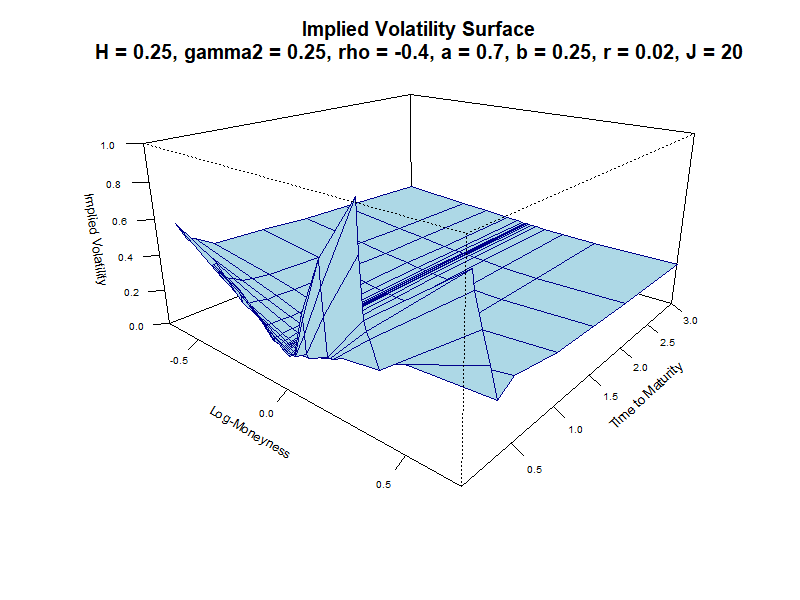
\includegraphics[width=0.45\textwidth]{figures/5.4 Optimal Parameter Ranges/optimal_example_iv_surface.png}
    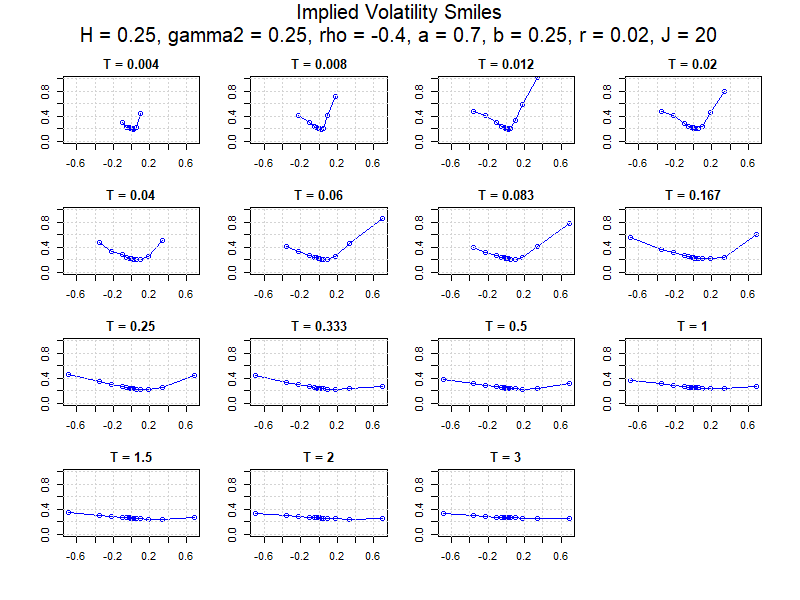
\includegraphics[width=0.45\textwidth]{figures/5.4 Optimal Parameter Ranges/optimal_example_iv_smiles.png}
    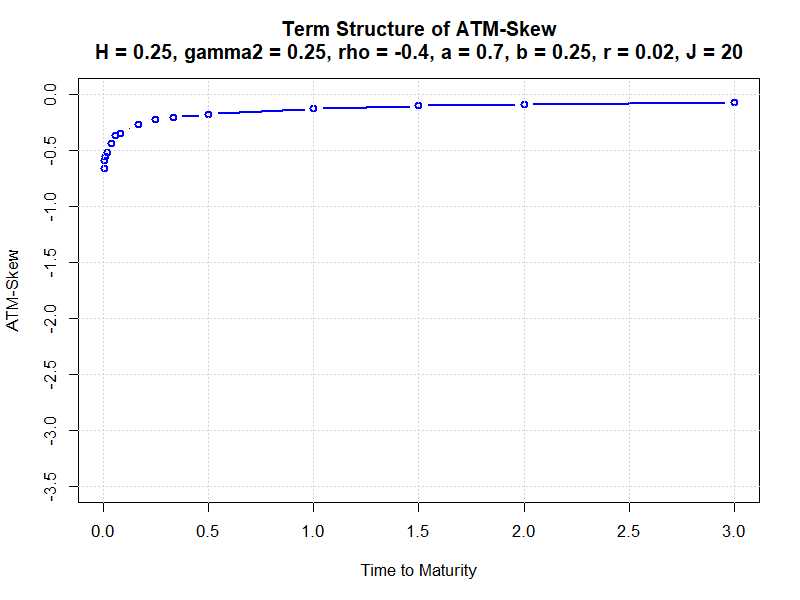
\includegraphics[width=0.45\textwidth]{figures/5.4 Optimal Parameter Ranges/optimal_example_atm_skew.png}
    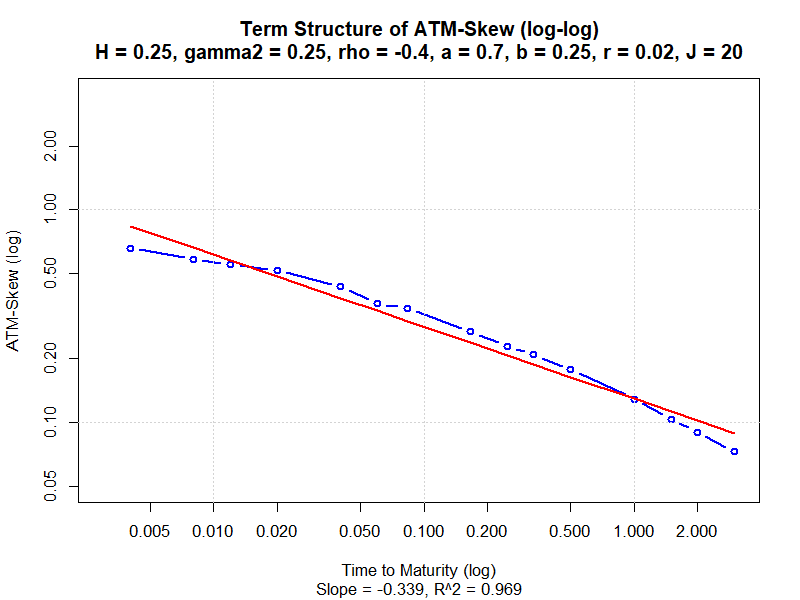
\includegraphics[width=0.45\textwidth]{figures/5.4 Optimal Parameter Ranges/optimal_example_atm_skew_log.png}
    \caption{Example implied volatility surface, smiles, ATM skew, and log-log skew term structure for an optimal parameter configuration.}
    \label{fig:OptimalExampleSurface}
\end{figure}

Figure~\ref{fig:OptimalExampleSurface} illustrates a surface generated with $H = 0.25$,  $\gamma_2 = 0.25$, $\rho = -0.4$, $a = 0.7$, $b = 0.25$, $r = 0.02$, and $J = 20$ (with $\gamma_1$ set according to Equation~\eqref{eq:HurstIndex}). This configuration satisfies all five criteria and produces a surface shape consistent with empirical market data.